\documentclass{beamer}
\usepackage{listings}
\lstset{
%language=C,
frame=single, 
breaklines=true,
columns=fullflexible
}
\usepackage{subcaption}
\usepackage{url}
\usepackage{tikz}
\usepackage{graphicx}
\usepackage{tkz-euclide} % loads  TikZ and tkz-base
%\usetkzobj{all}
\usetikzlibrary{calc,math}
\usepackage{float}
\usepackage{amsthm}
\usepackage{gensymb}
\newcommand\norm[1]{\left\lVert#1\right\rVert}
\renewcommand{\vec}[1]{\mathbf{#1}}
\newcommand{\R}{\mathbb{R}}
\newcommand{\C}{\mathbb{C}}
\newcommand{\comb}[2]{{}^{#1}\mathrm{C}_{#2}}
\providecommand{\brak}[1]{\ensuremath{\left(#1\right)}}
\providecommand{\abs}[1]{\vert#1\vert}
\providecommand{\fourier}{\overset{\mathcal{F}}{ \rightleftharpoons}}
\providecommand{\sbrak}[1]{\ensuremath{{}\left[#1\right]}}
\usepackage[export]{adjustbox}
\usepackage[utf8]{inputenc}
\usepackage{amsmath}
\DeclareMathOperator{\erfc}{erfc}
\usepackage[version=4]{mhchem}
\usetheme{Boadilla}
\title{Research Paper Presentation}
\author{C.Asish}
\institute{IITH}
\date{\today}
\begin{document}

\begin{frame}
\titlepage
\end{frame}
\begin{frame}{Title and Authors}
\begin{block}{Title}
A Morkov Model of Slice Admission Control
\end{block}
\begin{block}{Authors}
\begin{enumerate}
    \item Bin Han, Member,IEEE.
    \item Di Feng,Schotten, Member,IEEE.
    \item Hans D, Schotten, Member,IEEE.
\end{enumerate}
\end{block}
\end{frame}
\section{\textbf{Introduction}}
\subsection*{Index Terms}
\begin{frame}[fragile]
\frametitle{Index Terms}
\begin{enumerate}
    \item \textbf{Network slicing}: Network slicing is a method of creating multiple unique logical and virtualized networks over a common multidomain infrastructure. Each network slice is an isolated end to end network tailored to fulfil diverse requirements requested by a particular application 
    \item \textbf{state machine}: state machine is a behavior model which contains a finite number of states. Based on current state and a given input the machine performs state transitions and produce outputs 
    \item \textbf{Markov model}: In probability theory, Markov model is a stochastic model where the future states depend only on the current state, not on the events that occurred before it.
\end{enumerate}
\end{frame}

\begin{frame}{Abstract}
\begin{enumerate}
    \item The emerging feature of network slicing in future fifth generation networks calls for efficient slice management .
    \item  Recent studies have been focusing on the mechanism of slice admission control, which functions in a manner of state machine 
    \item This project proposes a general state model for synchronous slice admission control, and proves it to be Moravian under a set of weak constraints 
\end{enumerate}
\end{frame}

\begin{frame}{Introduction}
\begin{enumerate}
    \item Network slicing has been considered as an essential feature and one of the most important enablers of 5G cellular communications networks. It provides broad improvements of scalability, flexibility, accountability, shareabilty, and profitability to cellular networks 
    \item It allows mobile network operators (MNOs) to manage and utilize their physical and virtual network resources in the form of logically independent virtual mobile networks, a.k.a network slices.
    \item There are two types of inter-slice resource management First, when an MNO directly provides services to end users and maintains these services. Second, Slice as a service(SlaaS), MNO packs its resources into standardized atomic slices as and rents them to tenants such as virtual MNOs. 
    \item The SlaaS problem is more challenging due to stochastic nature and fluctuating behavior of tenant demand for resources 
\end{enumerate}
\end{frame}
\begin{frame}{System model}
\begin{block}{Resource allocation and Resource Feasibility}
\begin{enumerate}
    \item A Resource pool with M different types of countable resources can be described with the vector r = $[r_{1},r_{2},...,r_{M}]$. Consider N different slice types, for every bundle slice type n $\in[1,2,...,N]$ it costs a resource bundle $C_{n} =$ $[c_{1,n},c_{2,n},...,c_{M,n}]$ to maintain a slice which are atomic and indivisible.
    \item MNO manages its resources by adjusting set of active slides $s = [s_{1},s_{2},...s_{N}]$, where $s_{n}$  denotes the number of type -n slices under maintenance. The allocation is subjected to resource pool size :\\
    $r_{m}-\sum_{n=1}^{N}c_{m,n}s_{n}\geq 0$
\end{enumerate}
\end{block}
\end{frame}
\begin{frame}[fragile]
\frametitle{}
\begin{figure}
    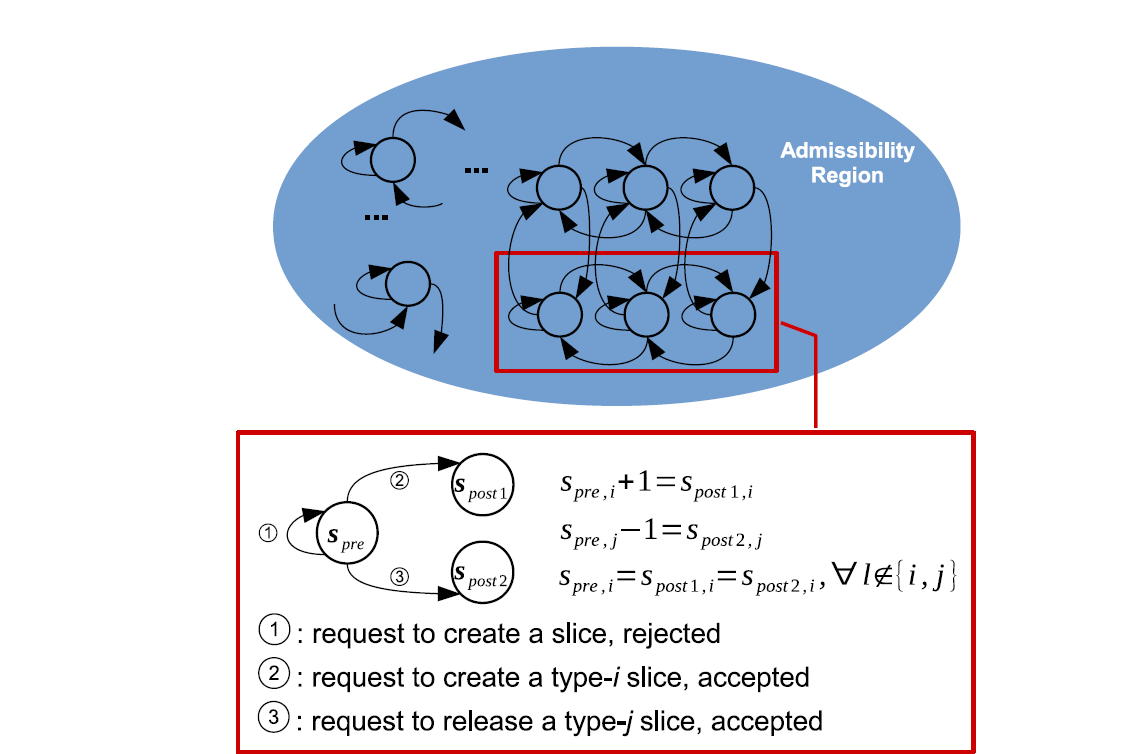
\includegraphics[scale=0.34]{fig-research.png}
    \caption{In asynchronous slice admission. the state is updated at request arrivals}
\end{figure}
\end{frame}

\begin{frame}{System model}
\begin{block}{Tenant Requests and Slice Admission Control}
\begin{enumerate}
    \item In SlaaS, slices are created and released upon requests from tenants.both the requests arrive randomly
   \item Generally defining the incoming request q and the MNO's binary decision d as\\
   q = 
\begin{cases}
   $n$ & $request to create a type -n slice$ \\
   $-n$ &  $request to release a type-n slice$\\
\end{cases}
\\
d =
\begin{cases}
   $1$ &  accepted(request)\\
   $0$ &   declined(request)
\end{cases}
 \item The post-transition state  $s_{post}$ is a function of q, d and the pre-transition state :\\
$s_{post}$ = T($s_{pre}$,q,d)
=[$s_{pre,1},...s_{pre,|q|}+d.sgn(q),...,s_{pre,N}$]
\end{enumerate}
\end{block}
\end{frame}
\begin{frame}{System model}
\begin{block}{Slicing strategy}
\begin{enumerate}
 \item If d is only a function of q and the pre-transition network state $s_{pre}$, we say that MNO has consistent slicing strategy d = D(q,$s_{pre}$)
 \item As MNO cannot overload the resource pool or decline to release slices\\
 D(q,s)=1,  $\forall q\in {-1,-2,.....,-N}$\\
 \item For any valid slicing strategy D, we have \\
 $s_{post}$=$T(s_{pre},q,D(q,s_{pre})) = T(s_{pre},q)$\\
\end{enumerate}
\end{block}
\end{frame}

\begin{frame}{Synchronous Slice Admission Control Model}
\begin{block}{Synchronous Slice Admission}
\begin{enumerate}
\item MNOs usually process requests in a framed approach, where all arrived requests, despite of the type will be buffered in queue sequentially responded at the end of every operation period.
\item Normalising the operation period length to 1, the MNO make sequential decisions to buffered requests at discrete time indexes, We use the vector q(t)=[$q_{1}(t),q_{2}(t),...,q_{Q_{t}}(t)$] to denote the request queue buffered during the $t^{th}$ operation ($Q_{t}$ is the total number of request ). the network state at  (t+1) is \\
\begin{align}
s(t+1) = T(...T(T( s(t), q_{1}(t), q_{2}(t),..., q_{Q_{t}}(t))= \hat{T}(s(t),q(t)),
\end{align}
\end{enumerate}
\end{block}
\end{frame}
\begin{frame}{Synchronous Slice Admission Control Model}
\begin{block}{Equivalent Markov Model}
We assume that type-n slice creation requests arrive as Poisson events in rate of $\lambda_{n}$, and that the lifetime of every type-n slice is an exponential random variable with mean of $\mu_{n}$\\
 the probability mass function that k$>$0 requests for type-n slice Creation q=n$>$0 arrive during one operation period is \\
\begin{align}
Prob(k_{n}) =  \frac{\lambda_{n}^{k_{n}}. e^{-\lambda_{n}}}{k_{n}\!}     n\in [1,2,...,N]
\end{align}
\end{block}
\end{frame}
\begin{frame}{Synchronous Slice Admission Control Model}
\begin{block}{Equivalent Markov Model}
 Given $s_{n}$ as the number of type-n slice under maintenance, the PMF that $0<k_{-n}\le s_{n}$ requests for type-n slice release $q=-n<0$ in the same operation is \\
\begin{lemma}
\begin{align}
   Prob(k_{-n} |s_{n}) = \frac {s_{n}!.(1- e^{-\frac{1}{\mu_{n}}})^{k_{-n}}}{k_{-n}!(s_{n}-k_{-n})!e^{\frac{s_n-k_-n}{\mu_n}  }}
 \end{align}
 \end{lemma}
\end{block}
\end{frame}

\begin{frame}{Synchronous Slice Admission Control Model}
\begin{block}{Equivalent Markov Model}
 \begin{proof}
 As request to release any of the  slice type-n is random and has unique chances(Binomial distribution), \\
 \begin{align}
 Prob(k_{-n} |s_{n})= {s_{n}\choose k_{-n}}          (p)^{k_{-n}}(1-p)^{s_{n}-k_{-n}}
 \end{align}
Here p is probability that slice types below n are released.\\
p = Pr(X$\le$x) = $1-e^{-\frac{1}{\mu_{n}}}$,  
 \end{proof}
\end{block}
\end{frame}

\begin{frame}{Synchronous Slice Admission Control Model}
\begin{block}{Equivalent Markov Model}
 We can merge them as \\
 \begin{align}
 P_{A}(k_{q},q | s_{|q|}) = 
     \begin{cases}
      \frac{\lambda_{q}^{k_{q}}. e^{-\lambda_{q}}}{k_{q}\!}  &  q>0\\
      \frac {s_{|q|}!(1- e^{-\frac{1}{\mu_{|q|}}})^{k_{q}}}{k_{q}!(s_{|q|}-k_{q})!e^{\frac{s_{|q|}-k_q}{\mu_{|q|}}  }}  & q<0
\end{cases}
 \end{align}
 We define $\hat{q}$ to denote the elements in a request sequence q regardless the order. Because the arrival process of different requests are independent from each other\\
\end{block}
\end{frame}

\begin{frame}{Synchronous Slice Admission Control Model}
\begin{block}{Equivalent Markov Model}
 The conditional probability that $\hat{q}$ arrives during one operation period in the current network state is \\
\begin{align}
 Prob(\hat{q}|s) = \prod_{q\in [\pm 1,...\pm N]}p_{A}(\sharp_{\hat{q}}^{q},q |s_{|q|}),
\end{align}
 where  $\sharp_{X}^{x}$ denotes the occurrence times of x in X\\
 As the arrival probability of a request sequence is independent of its order\\
 i.e Prob($q_{1}$ $|$ s) = Prob($q_{2}$ $|$ s), $\forall${$q_{1},q_{2}$} : $\hat q_{1}$ = $\hat q_{2}$\\
 so we have \\
 \begin{align}
Prob(\hat{q} | s) = \sum_{i:\hat{q}_{i}=\hat{q}} = Q!\times Prob(q|s),  
 \end{align}
\end{block}
\end{frame}

\begin{frame}{Synchronous Slice Admission Control Model}
\begin{block}{Equivalent Markov Model}
 Where Q is the length of q. This yields that \\
    \begin{align}
      Prob(q|s) = \frac{\prod_{q\in [\pm 1,...\pm N]}p_{A}(\sharp_{\hat{q}}^{q},q |s_{|q|})}{Q!},
    \end{align}
    Now calling back (1), we are able to obtain the synchronous transition probability from state s(t) to s(t+1) as\\
    \begin{align}
        Prob(s(t+1)|s(t)) = \sum_{q:\hat{T}(s(t),q)= s(t+1)} Prob(q|s(t)),
    \end{align}
    which depends only on s(t). The synchronous slice management process is therefore Markovian. 
\end{block}
\end{frame}
\begin{frame}{Conclusions}
\begin{enumerate}
    \item When the  statistics of request arrivals are memoryless, e.g., when they are Poisson or exponential processes, and when the MNO takes a consistent slicing strategy, the state model is Markovian.
    \item The Markov model of network state is individually determined by the applied slicing strategy. This guarantees that optimization problems of slice admission can be equivalently transformed into the problem of searching the best slicing strategy.  
 
\end{enumerate}
\end{frame}
\end{document}